\documentclass[tikz,border=6pt]{standalone}
\usepackage[T1]{fontenc}
\usepackage{tgpagella}
\usepackage{tikz}
\usetikzlibrary{arrows.meta, calc, positioning}

\definecolor{ink}{HTML}{23313B}
\definecolor{muted}{HTML}{6B747C}
\definecolor{line}{HTML}{CAD1D6}
\definecolor{paper}{HTML}{F5F2EC}
\definecolor{c1}{HTML}{335C81}
\definecolor{c2}{HTML}{2D7A78}
\definecolor{c3}{HTML}{4B7A4F}
\definecolor{c4}{HTML}{9B7A2E}
\definecolor{c5}{HTML}{A15B50}
\definecolor{c6}{HTML}{7A4E73}

\begin{document}
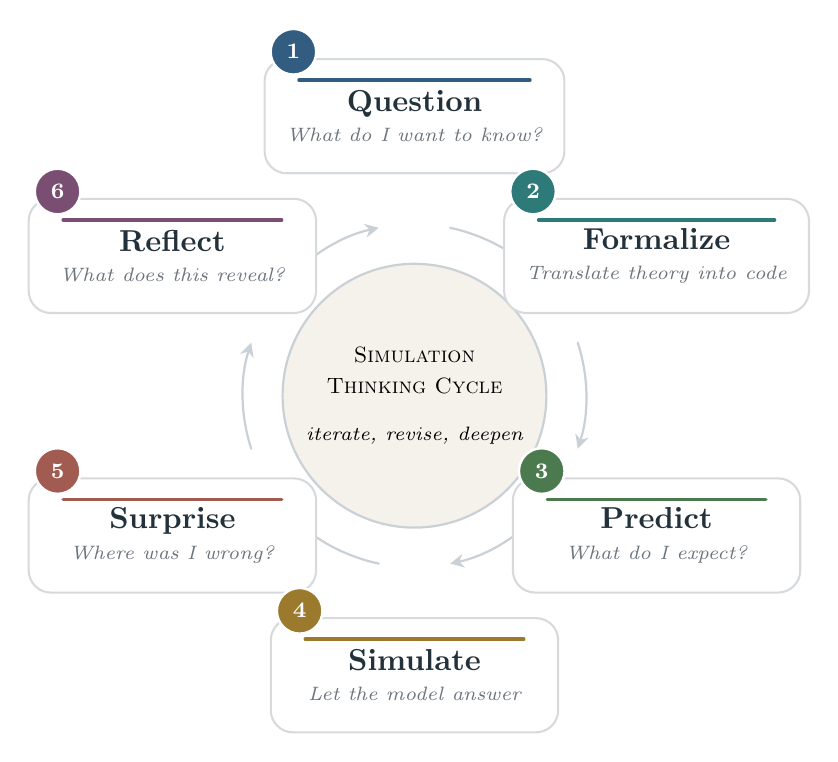
\begin{tikzpicture}[
    font=\rmfamily,
    flow/.style={
      draw=line,
      line width=0.8pt,
      -{Stealth[length=5pt,width=5pt]},
      line cap=round,
    },
    card/.style={
      draw=ink!18,
      fill=white,
      rounded corners=8pt,
      line width=0.75pt,
      minimum width=3.65cm,
      minimum height=1.45cm,
      inner sep=8pt,
      align=center,
    },
    badge/.style={
      circle,
      fill=#1,
      draw=white,
      line width=0.9pt,
      minimum size=5.8mm,
      inner sep=0pt,
      font=\bfseries\footnotesize,
      text=white,
    },
    accent/.style={
      draw=#1,
      line width=1.2pt,
      line cap=round,
    },
  ]

  \def\R{3.55cm}
  \def\Ring{2.18cm}

  % Clockwise flow ring
  \foreach \start/\stop in {78/42,18/-18,-42/-78,-102/-138,-162/-198,138/102} {
    \draw[flow] (\start:\Ring) arc[start angle=\start, end angle=\stop, radius=\Ring];
  }

  % Centre
  \node[
    circle,
    draw=line,
    line width=0.8pt,
    fill=paper,
    minimum size=3.35cm,
    align=center
  ] (core) at (0,0) {%
    {\fontsize{8.2}{9.0}\selectfont\textsc{Simulation}}\\[-1pt]
    {\fontsize{8.2}{9.0}\selectfont\textsc{Thinking Cycle}}\\[5pt]
    {\itshape\fontsize{7.4}{8.2}\selectfont iterate, revise, deepen}
  };

  % Step cards
  \node[card] (Q) at (90:\R) {%
    {\bfseries\fontsize{10.5}{11.5}\selectfont\color{ink} Question}\\[-1pt]
    {\itshape\fontsize{7.4}{8.4}\selectfont\color{muted} What do I want to know?}
  };
  \node[card] (F) at (30:\R) {%
    {\bfseries\fontsize{10.5}{11.5}\selectfont\color{ink} Formalize}\\[-1pt]
    {\itshape\fontsize{7.4}{8.4}\selectfont\color{muted} Translate theory into code}
  };
  \node[card] (P) at (330:\R) {%
    {\bfseries\fontsize{10.5}{11.5}\selectfont\color{ink} Predict}\\[-1pt]
    {\itshape\fontsize{7.4}{8.4}\selectfont\color{muted} What do I expect?}
  };
  \node[card] (S) at (270:\R) {%
    {\bfseries\fontsize{10.5}{11.5}\selectfont\color{ink} Simulate}\\[-1pt]
    {\itshape\fontsize{7.4}{8.4}\selectfont\color{muted} Let the model answer}
  };
  \node[card] (X) at (210:\R) {%
    {\bfseries\fontsize{10.5}{11.5}\selectfont\color{ink} Surprise}\\[-1pt]
    {\itshape\fontsize{7.4}{8.4}\selectfont\color{muted} Where was I wrong?}
  };
  \node[card] (R) at (150:\R) {%
    {\bfseries\fontsize{10.5}{11.5}\selectfont\color{ink} Reflect}\\[-1pt]
    {\itshape\fontsize{7.4}{8.4}\selectfont\color{muted} What does this reveal?}
  };

  % Accent rules
  \draw[accent=c1] ($(Q.north west)+(0.45cm,-0.28cm)$) -- ($(Q.north east)+(-0.45cm,-0.28cm)$);
  \draw[accent=c2] ($(F.north west)+(0.45cm,-0.28cm)$) -- ($(F.north east)+(-0.45cm,-0.28cm)$);
  \draw[accent=c3] ($(P.north west)+(0.45cm,-0.28cm)$) -- ($(P.north east)+(-0.45cm,-0.28cm)$);
  \draw[accent=c4] ($(S.north west)+(0.45cm,-0.28cm)$) -- ($(S.north east)+(-0.45cm,-0.28cm)$);
  \draw[accent=c5] ($(X.north west)+(0.45cm,-0.28cm)$) -- ($(X.north east)+(-0.45cm,-0.28cm)$);
  \draw[accent=c6] ($(R.north west)+(0.45cm,-0.28cm)$) -- ($(R.north east)+(-0.45cm,-0.28cm)$);

  % Number badges
  \node[badge=c1] at ($(Q.north west)+(0.38cm,0.08cm)$) {1};
  \node[badge=c2] at ($(F.north west)+(0.38cm,0.08cm)$) {2};
  \node[badge=c3] at ($(P.north west)+(0.38cm,0.08cm)$) {3};
  \node[badge=c4] at ($(S.north west)+(0.38cm,0.08cm)$) {4};
  \node[badge=c5] at ($(X.north west)+(0.38cm,0.08cm)$) {5};
  \node[badge=c6] at ($(R.north west)+(0.38cm,0.08cm)$) {6};

\end{tikzpicture}
\end{document}
